% !TEX root = ../report_v2.tex
\appendix
\section*{Appendices}
\addcontentsline{toc}{section}{Appendices}
\renewcommand{\thesubsection}{\Alph{subsection}}

\subsection{Application Repository}
\label{appendix:code}
https://github.com/StephenCoady/lifecycle-management-for-docker

\subsection{Travis Repository} 
\label{appendix:travis}
https://travis-ci.org/StephenCoady/lifecycle-management-for-docker

\subsection{SonarQube Repository} 
\label{appendix:sonarqube}
https://sonarqube.com/dashboard/index?id=lifecyle-management-for-docker

\subsection{DockerHub Repository} 
\label{appendix:dockerhub}
https://hub.docker.com/r/scoady2/lifecycle-management-for-docker/

\subsection{Staging Server} 
\label{appendix:staging}
application: http://87.44.18.55:3000/
documentation: http://87.44.18.55/docs

default username: admin \newline
default password: admin

\subsection{Dockerode} 
\label{appendix:dockerode_appendix}
https://github.com/apocas/dockerode

\subsection{Report Source Code} 
\label{appendix:reports}
https://github.com/StephenCoady/fyp-documentation

\subsection{Sprint Retrospectives}
\label{appendix:retros}
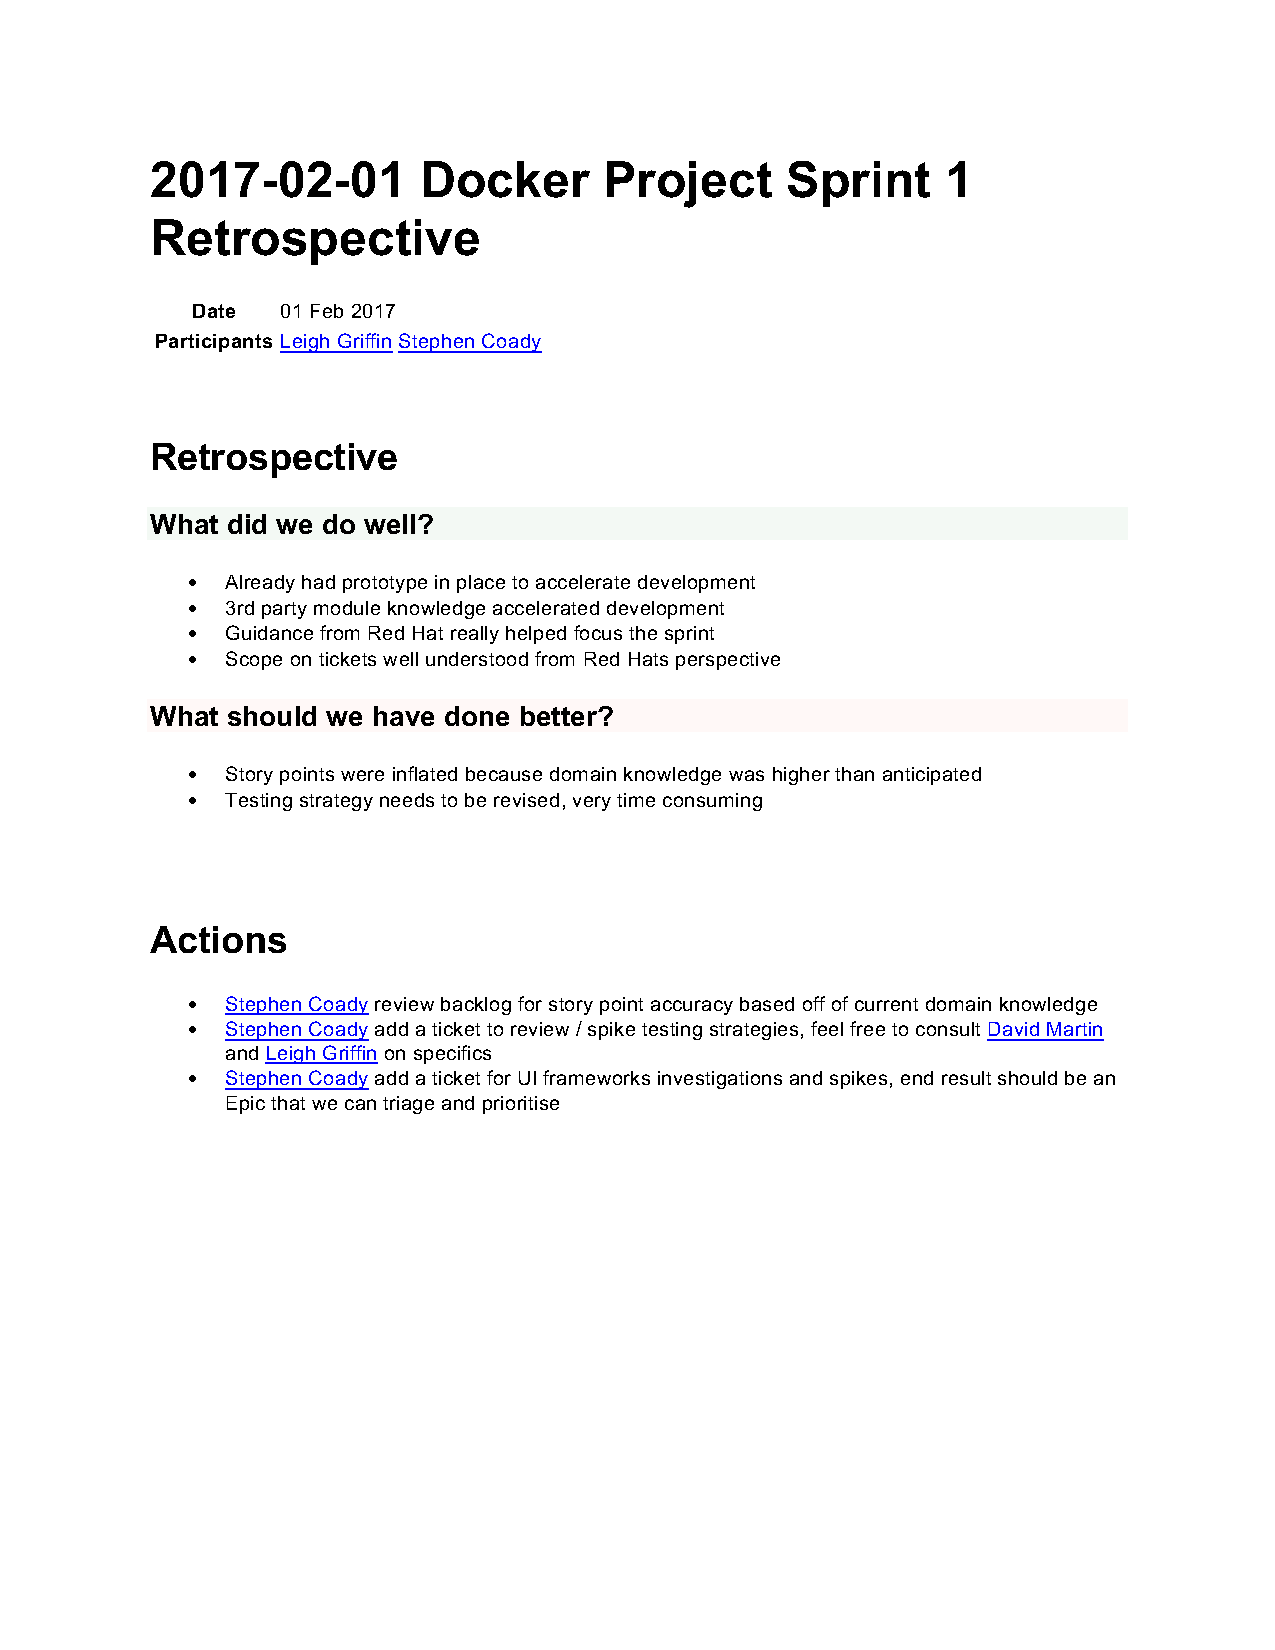
\includepdf[pages=-,pagecommand={}]{components/retrospectives/sprint_1_retrospective.pdf}
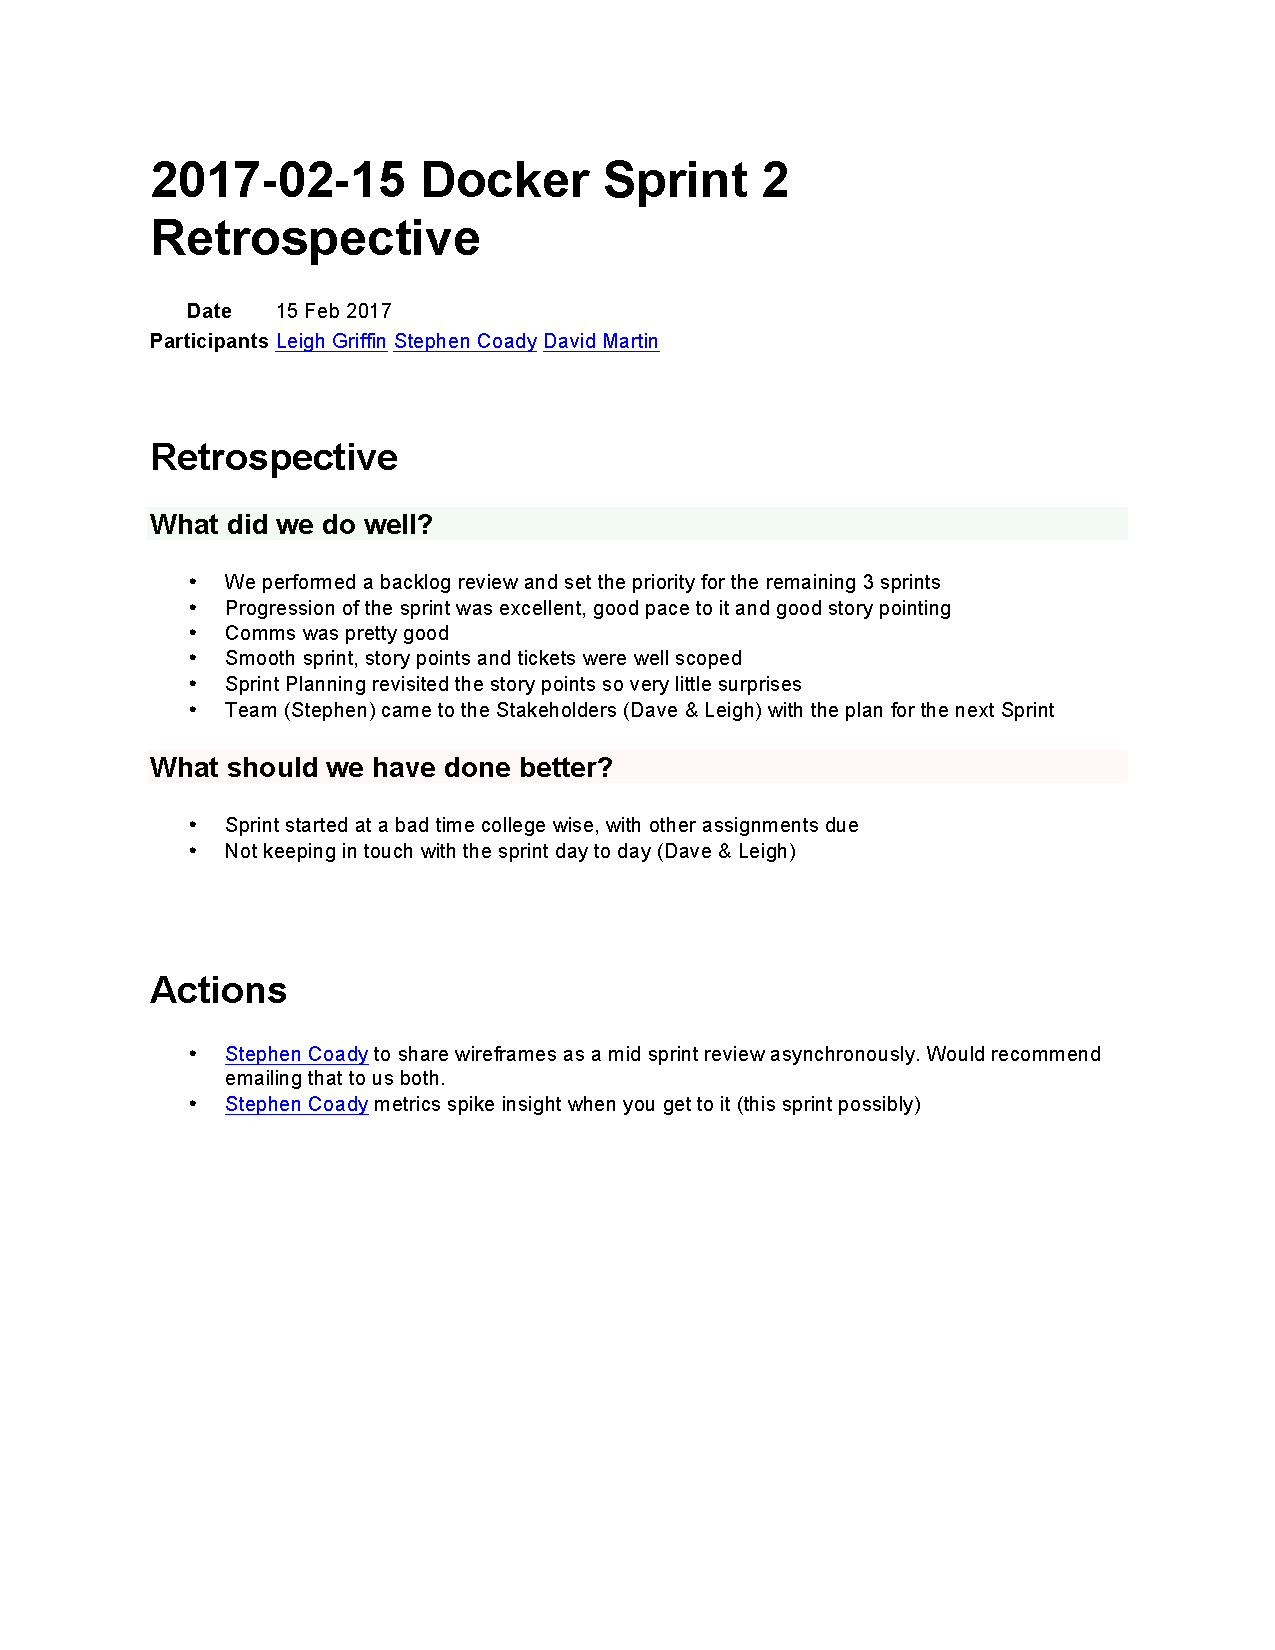
\includepdf[pages=-,pagecommand={}]{components/retrospectives/sprint_2_retrospective.pdf}
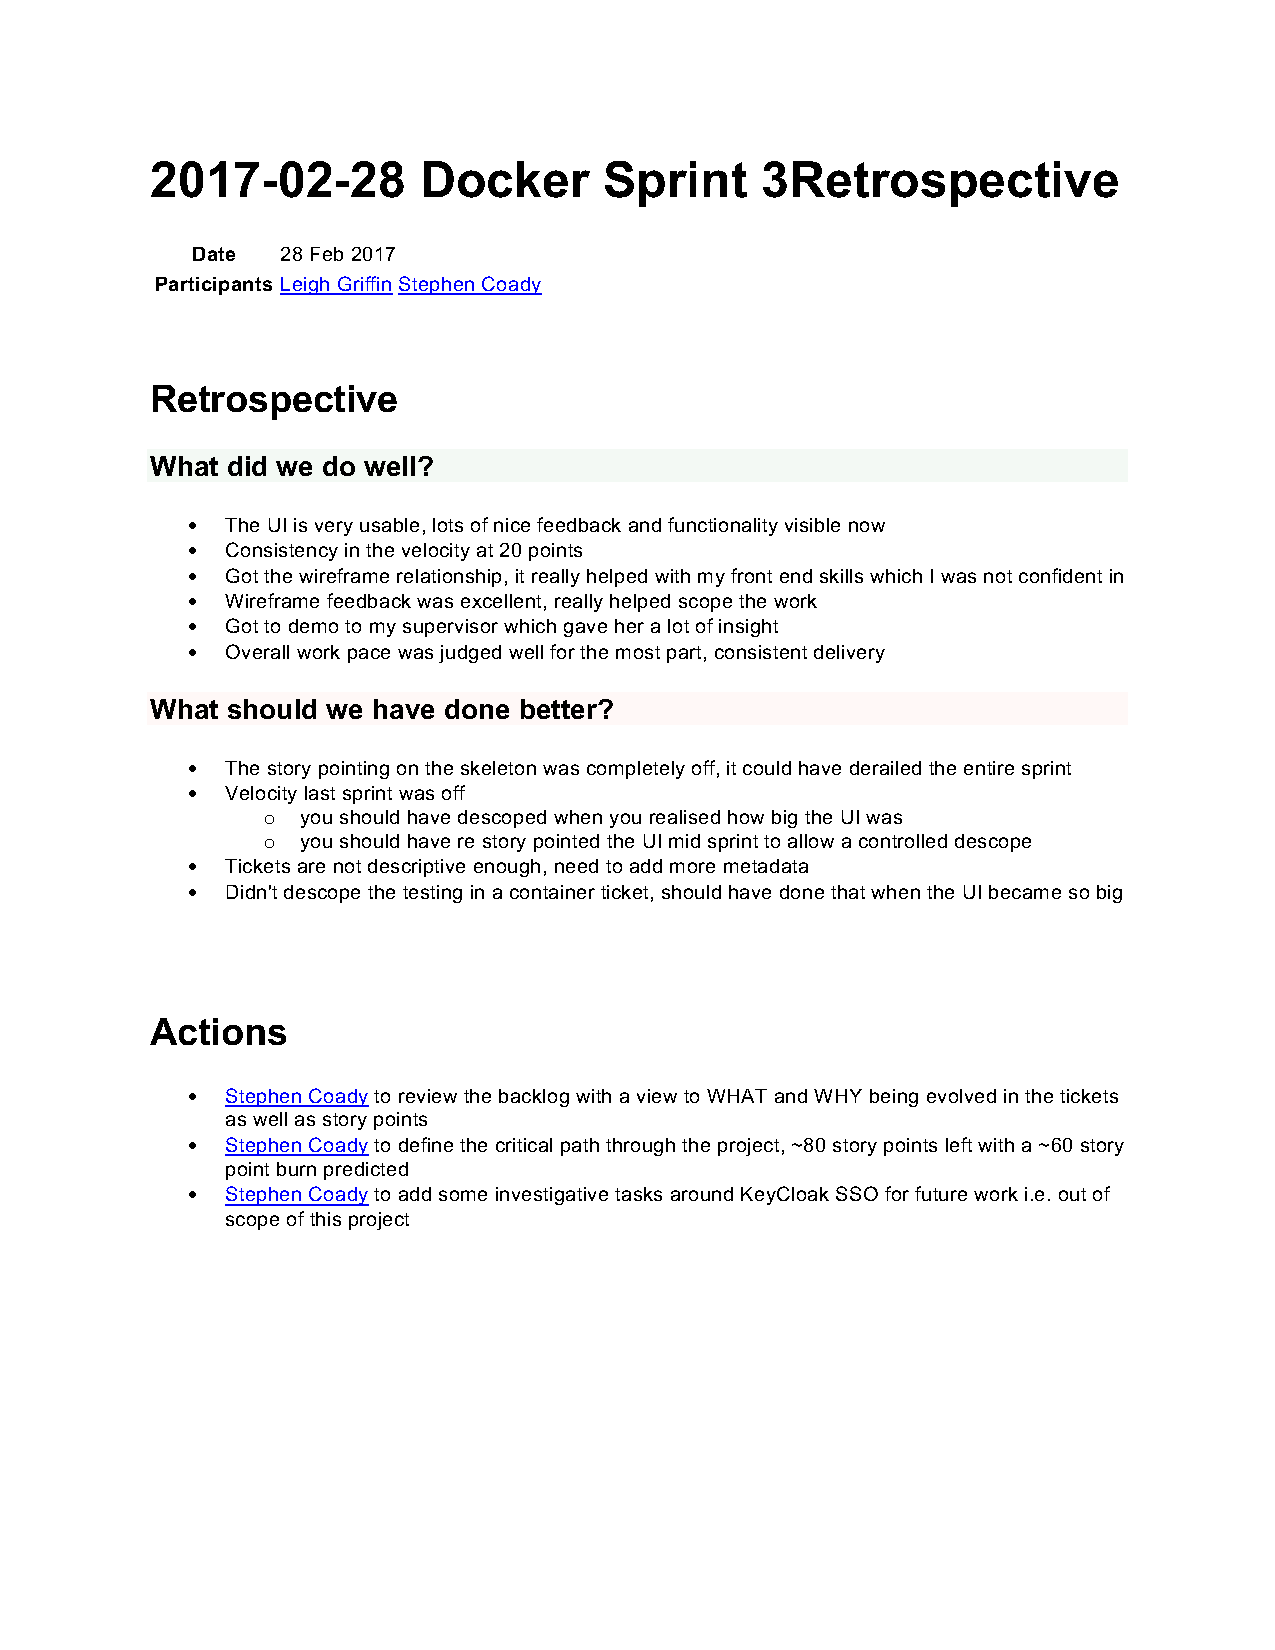
\includepdf[pages=-,pagecommand={}]{components/retrospectives/sprint_3_retrospective.pdf}
\clearpage

\subsection{Formal System Models}
\label{appendix:models}

\begin{figure}[!ht]
\centering
\makebox[\textwidth]{\includegraphics*[width=0.9\paperwidth]{images/models/docker_class_diagram}}
\caption{\em Class Diagram}
\end{figure}

\begin{figure}[!ht]
\centering
\makebox[\textwidth]{\includegraphics*[width=0.9\paperwidth]{images/models/docker_system}}
\caption{\em Sequence Diagram}
\end{figure}

\begin{figure}[!ht]
\centering
\makebox[\textwidth]{\includegraphics*[width=0.8\paperwidth]{images/models/user_system}}
\caption{\em User System Sequence Diagram}
\end{figure}

\begin{figure}[!ht]
\centering
\makebox[\textwidth]{\includegraphics*[width=0.9\paperwidth]{images/models/use_case}}
\caption{\em Use Case Diagram}
\end{figure}

\subsection{Wireframes}
\label{appendix:wireframes}

\begin{figure}[!ht]
\centering
\includegraphics*[width=0.9\textwidth]{wireframes/dashboard}
\caption{\em Dashboard Mockup}
\end{figure}

\begin{figure}[!ht]
\centering
\includegraphics*[width=0.9\textwidth]{wireframes/container}
\caption{\em Container Mockup}
\end{figure}

\begin{figure}[!ht]
\centering
\includegraphics*[width=0.9\textwidth]{wireframes/images}
\caption{\em Images Mockup}
\end{figure}

\begin{figure}[!ht]
\centering
\includegraphics*[width=0.9\textwidth]{wireframes/image}
\caption{\em Image Mockup}
\end{figure}

\begin{figure}[!ht]
\centering
\includegraphics*[width=0.9\textwidth]{wireframes/networks}
\caption{\em Networks Mockup}
\end{figure}

\begin{figure}[!ht]
\centering
\includegraphics*[width=0.9\textwidth]{wireframes/network}
\caption{\em Network Mockup}
\end{figure}

\begin{figure}[!ht]
\centering
\includegraphics*[width=0.9\textwidth]{wireframes/docker}
\caption{\em Docker Mockup}
\end{figure}

\begin{figure}[!ht]
\centering
\includegraphics*[width=0.9\textwidth]{wireframes/host}
\caption{\em Host Mockup}
\end{figure}
